\documentclass[article,10pt]{scrartcl}
\usepackage{graphicx}
\usepackage{amsmath}
\usepackage{tikz}
\usepackage{vmargin}
\setmarginsrb{1.3cm}{1.3cm}{1.3cm}{1.3cm}{1.3cm}{1.3cm}{1.3cm}{1.3cm}
\setlength{\parindent}{0cm}
\usepackage{color}
\usepackage{listings}
\usepackage{hyperref}
\usepackage[final]{pdfpages}
% python script syntax taken from 
% http://widerin.org/blog/syntax-highlighting-for-python-scripts-in-latex-documents
\definecolor{Code}{rgb}{0,0,0}
\definecolor{Decorators}{rgb}{0.5,0.5,0.5}
\definecolor{Numbers}{rgb}{0.5,0,0}
\definecolor{MatchingBrackets}{rgb}{0.25,0.5,0.5}
\definecolor{Keywords}{rgb}{0,0,1}
\definecolor{self}{rgb}{0,0,0}
\definecolor{Strings}{rgb}{0,0.63,0}
\definecolor{Comments}{rgb}{0,0.63,1}
\definecolor{Backquotes}{rgb}{0,0,0}
\definecolor{Classname}{rgb}{0,0,0}
\definecolor{FunctionName}{rgb}{0,0,0}
\definecolor{Operators}{rgb}{0,0,0}
\definecolor{Background}{rgb}{0.98,0.98,0.98}
\lstnewenvironment{python}[1][]{
\lstset{
%numbers=left,
%numberstyle=\footnotesize,
%numbersep=1em,
xleftmargin=1em,
framextopmargin=2em,
framexbottommargin=2em,
showspaces=false,
showtabs=false,
showstringspaces=false,
frame=l,
tabsize=4,
% Basic
%basicstyle=\ttfamily\small\setstretch{},
backgroundcolor=\color{Background},
language=Python,
% Comments
commentstyle=\color{Comments}\slshape,
% Strings
stringstyle=\color{Strings},
morecomment=[s][\color{Strings}]{"""}{"""},
morecomment=[s][\color{Strings}]{'''}{'''},
% keywords
morekeywords={import,from,class,def,for,while,if,is,in,elif,else,not,and,or,print,break,continue,return,True,False,None,access,as,,del,except,exec,finally,global,import,lambda,pass,print,raise,try,assert},
keywordstyle={\color{Keywords}\bfseries},
% additional keywords
morekeywords={[2]@invariant},
keywordstyle={[2]\color{Decorators}\slshape},
emph={self},
emphstyle={\color{self}\slshape},
%
}}{}

\begin{document}
\title{Basic programming with Python}
\subtitle{Student and Staff IT Introduction}
\date{25/06/2013}
\author{ssiti2013@gmail.com\footnote{Document written by Elsa Guillot (e.guillot@massey.ac.nz), for IFS staff and students, Massey University.}}
\maketitle
\section{Programming?}
Programming is the key to a whole new world: 
\begin{itemize}
\item Make simple computer task automatic
\item Become the master of your own analyses
\item Make your analyses automatic
\item Simulate data
\item Answer new research questions
\end{itemize}
All this is more accessible than you think!




\section{Programming languages: opening the black box}

Software that you usually use are black boxes. You input data, select a few parameters, and let the magic operates. Today we are going to open the black box\footnote{This is a simplified version of the theory of programming languages. The field is actually animated by fierce debate on the different definitions of languages, difference between interpreted and compiled, etc. None of which is meaningful for the purpose of this introduction}.
\\
Your computer speaks and operates in term of $0$ and $1$. A programming language is a way to communicate with the computer, make it compute your instructions (calculation, algorithm, file treatment), using a language understandable by humans and that can ultimately be translated into $0$ and $1$ to the computer.\\
 Programming languages fall into two different categories: interpreted languages and compiled languages. Using an interpreted language, such as Python, you speak to an Interpreter which answers immediately to you --- ``on the fly''. You can communicate to the interpreter directly in command lines or via scripts. If you write a program in a compiled language however, you will have to write a code in a text file and compile it using another program. This will transform your text file into an executable, i.e. a program that will be ready to run. 

\tikzstyle{black-box} = [rectangle, draw, fill=black!20, text width=11em, text centered, minimum height=5em]
\begin{figure}[h!]
\begin{center}
\begin{tikzpicture}[scale=0.8]
  \node (A) at (0,0) {Command};
  \node[black-box] (B) at (5,0) {Interpreter};
  \node (C) at (10,0) {Output};
  \draw[black,->] (A) -- (B);
  \draw[black,->] (B) -- (C);
\end{tikzpicture}
\end{center}
\caption{Programming with an interpreted language}
\end{figure}
\begin{figure}[h!]
\begin{center}
\begin{tikzpicture}[scale=0.8]
  \node (A) at (0,0) {Code script};
  \node[black-box] (B) at (5,0) {Compiler};
  \node (C) at (10,0) {Executable};
  \draw[black,->] (A) -- (B);
  \draw[black,->] (B) -- (C);
\end{tikzpicture}
\end{center}
\caption{Programming with a compiled languages}
\end{figure}
\begin{center}
\begin{tabular}{|l|l|l|}
\hline
Language & Compiled / Interpreted & Object oriented\\ 
\hline 
FORTRAN & compiled & FORTRAN 2003 \\
\hline
C & compiled & No\\
\hline
C++ & compiled & Yes\\
\hline
C\# & compiled & Yes \\
\hline
Python & Interpreted & Yes \\
\hline
Java &  Interpreted & Yes \\
\hline
Ruby & Interpreted & Yes \\
\hline
Perl & Interpreted & from version 5\\
\hline
R & Interpreted & Yes\\
\hline
PHP & Interpreted & From PHP 3\\
\hline
\end{tabular}
\end{center}

In Bioinformatics, two languages are dominating in the programming of data analyses scripts : Python and Perl. Both are called ``scripting languages'' and are very similar in what they can do, but the battle is fierce between the pro-Python and the pro-Perl.

\begin{center}
\begin{tabular}{|c|cc|}
\hline
& Python & Perl\\
\hline
Creation year & 1991 & 1987\\
Syntax & Simple & Complex and cryptic\\
Power & Vast amount of libraries & Rich in operator symbol \\
\hline
\end{tabular}
\end{center}

\begin{figure}[h!]
\begin{center}
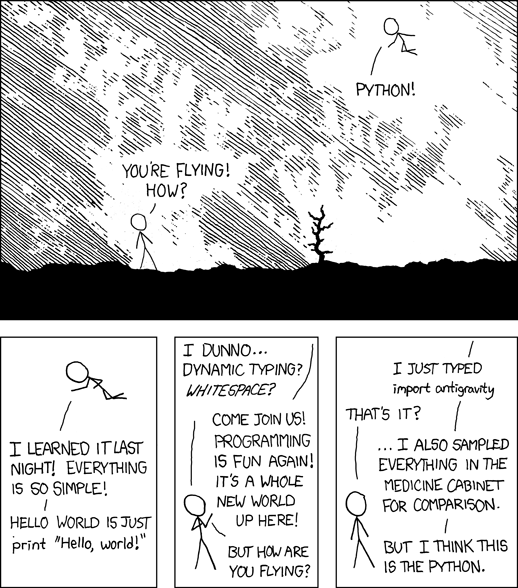
\includegraphics[scale=0.3]{xkcd_python.png}\\
\url{http://xkcd.com/353/}
\end{center}
\end{figure}


\section{Python programming}
Python is an easy language to learn and practice. \\
Open a shell :\\
\texttt{\$ python}\\
You are now in the python interpreter, any command that you will type will be interpreted into python. As a tradition in computer science, we will start by making the computer says ``Hello World'' :\\
\texttt{>>> print(``Hello World'')}\\
\texttt{Hello World}\\
\texttt{>>> print('I print what I want')}\\
\texttt{I print what I want}\\
\texttt{>>> print 42}\\
\texttt{42}\\
\texttt{>>>\#this is a comment}\\
\\
Python knows mathematics:\\
\texttt{>>> 1+1}\\
\texttt{2}\\
\texttt{>>> 36-7}\\
\texttt{29}\\
\texttt{>>> 21*2}\\
\texttt{42}\\
\texttt{>>> 42/2}\\
\texttt{21}\\


Call previous commands : up-arrow.\\
Quit python:\\
\texttt{>>>exit()}\\
You are back to the main shell. Type python to go back in the interpreter:\\
\texttt{\$python}\\
All the documentation you need to program in python is on this website \url{http://docs.python.org/2.6/}
\subsection*{Variables !}
A variable is an object in which you store a value.\\
\texttt{>>> myvalue = 42}\\
\texttt{>>> myothervalue = ``Hello world''}\\
\texttt{>>> myvalue}\\
\texttt{42}\\
\texttt{>>> myothervalue}\\
\texttt{``Hello world''}\\
\texttt{>>> a=1 \# save value 1 into a}\\
\texttt{>>> b=2}\\
\texttt{>>> a+b}\\
\texttt{3}\\
\texttt{>>> c=a+b+b}\\
\texttt{>>> c}\\
\texttt{5}\\
\texttt{>>> b=3 \# modify the value of b}\\
\texttt{>>> b}\\
\texttt{3}\\
\texttt{>>> a=c \# copy the value of c to a}\\
\texttt{>>> a}\\
\texttt{5}\\
\\
Each value has a type, which will define what you can do with it. Python handles the type of your variable for you.\\
\texttt{>>> type(myvalue)}\\
\texttt{<type 'int'>}\\
\texttt{>>> type(myothervalue)}\\
\texttt{<type 'str'>}


\begin{tabular}{|c|c|c|c|}
\hline
type & abbreviation &  null value & example \\
\hline
boolean & bool &  False & False\\ 
\hline
integer & int &  0 & 42 \\
\hline
floating point & float & 0.0 & 1.5 \\
\hline
complex & complex &  0j & 4+2j\\
\hline
string & str &  '' & 'Hello World'\\
\hline
list & list &  [] & [0,1,2,3] \\
& & & ['a','b','cde',42]\\
\hline
tuple & tuple &  () & (42,'hello world')\\
\hline
dictionary & dict &  \{\} & \{'English':'Hello world',\\
&&&'French':'Bonjour tout le monde',\\
&&&'computer':'0011001101'\}\\
\hline
\end{tabular}\\

There exist a type called \textbf{tuple}. It is used to send a small set of values to and from functions.\\

We ignore two more types \textit{set} and \textit{frozenset} for now.\\


Why does it matter to know the type then ?\\
\texttt{>>> 1 \# this is an integer}\\
\texttt{1}\\
\texttt{>>> 1.0 \# this is a float}\\
\texttt{1.0}\\
\texttt{>>> '1' \# this is a string}\\
\texttt{'1'}\\
\texttt{>>> 1+1 }\\
\texttt{2 }\\
\texttt{>>> 1+1.0 \# adding an integer and a float gives you a float}\\
\texttt{2.0 }\\
\texttt{>>> 1+'1' \# you can not add an integer to a string }\\
\texttt{TypeError }\\
\texttt{>>> '1'+'1' \# adding string concatenate them}\\
\texttt{'11' }\\
\texttt{>>> 43/2}\\
\texttt{21}\\
\texttt{>>> 43.0/2}\\
\texttt{21.5}\\
\texttt{>>> 43/2.0}\\
\texttt{21.5}\\
\\
The operation of adding string is called string concatenation. It is extremely useful:
\texttt{>>> 'Hello'+' '+'fellow programmers' \# adding string concatenate them}\\
\texttt{'Hello fellow programmers' }\\

\texttt{>>>mylist=['a','b','c','d','e']}\\
\texttt{>>>mylist[0] \# access the first cell}\\

\textbf{In python, as in C and C++, for example, the first element of the cell has index 0}\\

\texttt{'a'}\\
\texttt{>>>mylist.index('a') \# find the index of the first cell containing 'a'}\\
\texttt{0}\\
\texttt{>>>mylist[2]}\\
\texttt{'c'}\\
\texttt{>>>mylist[1:4] \# access cell 1, 2 and 3}\\
\texttt{['b','c','d']}\\
\texttt{>>>mylist[-1]}\\
\texttt{'e'}\\
\texttt{>>>mylist}\\
\texttt{['a','b','c','d','e']}\\
\texttt{>>>mylist.append('f') \# add a cell at the end with value f}\\
\texttt{>>>mylist}\\
\texttt{['a','b','c','d','e','f']}\\
\texttt{>>>mylist.pop() \# delete last cell}\\
\texttt{>>>mylist}\\
\texttt{['a','b','c','d','e']}\\
\texttt{>>>mylist.pop(0) \# delete cell 0}\\
\texttt{>>>mylist}\\
\texttt{['b','c','d','e']}\\
\texttt{>>>mylist2=['Hello','world']}\\
\texttt{>>>mylist2}\\
\texttt{['Hello','world']}\\
\texttt{>>>mylist+mylist2 \# concatenate lists}\\
\texttt{['b','c','d','e','Hello','world']}\\

To keep on exploring the list, try to play with the commands \textit{mylist.reverse(), mylist.count(), mylist.index(), mylist.insert(), mylist.remove(), mylist.sort(), mylist.extend()}\\
Use python help :\\
\texttt{>>>help(list.reverse)}\\
\textbf{When calling the help of a function, do not write the parenthesis!}

The dictionary are very similar to list, except that you access the values using keys:\\
\texttt{>>>mydict=\{'key':'value','english':'hello','french':'bonjour'\} \# create the dictionary}\\
\texttt{>>>mydict['english']}\\
\texttt{'hello'}\\
\texttt{>>>mydict.keys() \# list the keys}\\
\texttt{['french', 'key', 'english']}\\
\texttt{>>>mydict.values() \#list the values}\\
\texttt{['bonjour', 'value', 'hello']}\\
\texttt{>>>mydict.pop('key') \# remove the entry 'key' and its value 'value'}\\
\texttt{['value']}\\
\texttt{>>>mydict['spanish']='hola' \# add a new entry}\\
Dictionaries have plenty of functions to handle them, you can see the list using the help :\\
\texttt{>>>help(dict)}\\

Strings have specific functions too. You can access each letter as if it was an array:
\texttt{>>>a='hello'}\\
\texttt{>>>a[1]}\\
\texttt{'e'}\\
You can also find letters in the string (using \textbf{find()}), count the number of occurrence of a letter (\textbf{count()}), check if the string represent an integer (\textbf{isdigit()}), change the text into capital letters (\textbf{upper()}) or lower ones (\textbf{lower}). Look at the \textbf{help(str)} for a full description.\\
A useful function on the string is the function \textbf{split('x')}. It will find all the occurrence of \textbf{'x'} in the string, and make a list out of all the elements between the \textbf{'x'}. The result will be a list of n+1 elements, if n is the number of occurrences of \textbf{'x'} (x can be a single character or a string itself).\\
\texttt{>>>a='hello my fellow'}\\
\texttt{>>>a.split('y')}\\
\texttt{['hello m', ' fellow']}\\
\texttt{>>>a.split('l')}\\
\texttt{['he', '', 'o my fe', '', 'ow']}\\
\texttt{>>>a.split()}\\
\texttt{['hello', 'my','fellow']}\\
By default (i.e. without argument), \textbf{split} will separate the string where empty spaces are found.\\


Finally it is possible to change the type of a variable, using \textbf{int()}, \textbf{str()}, \textbf{float()}:\\
\texttt{>>>a=1}\\
\texttt{>>>a}\\
\texttt{1}\\
\texttt{>>>b=str(a)}\\
\texttt{>>>b}\\
\texttt{'1'}\\
\texttt{>>>c=float(b)}\\
\texttt{>>>c}\\
\texttt{1.0}\\
\texttt{>>>d=float(a)}\\
\texttt{>>>d}\\
\texttt{1.0}\\
\texttt{>>>f=int(b)}\\
\texttt{>>>f}\\
\texttt{1}\\

\textbf{Be careful when you copy a variable !} There is great danger with copy, and you may not even know that you doing copies. A copy is the transfer of value from one variable to another. For example, here b will be a copy of a:\\
\texttt{>>>a=1}\\
\texttt{>>>b=a}\\
\texttt{>>>b}\\
\texttt{1}\\
With integers, float and string, there are no problem. You copy, and then each variable is independent.\\
\texttt{>>>a=1}\\
\texttt{>>>b=a}\\
\texttt{>>>b=36}\\
\texttt{>>>b}\\
\texttt{36}\\
\texttt{>>>a}\\
\texttt{1}\\

With list however, when you copy a variable using \textbf{=} there is dependency between the variable: they will refer to the same set of elements. It is problematic because if you modify one, you will also modify the other:\\
\texttt{>>>a=range(10)}\\
\texttt{>>>a}\\
\texttt{[0, 1, 2, 3, 4, 5, 6, 7, 8, 9]}\\
\texttt{>>>b=a}\\
\texttt{>>>b}\\
\texttt{[0, 1, 2, 3, 4, 5, 6, 7, 8, 9]}\\
\texttt{>>>a[1]=42}\\
\texttt{>>>a}\\
\texttt{[0, 42, 2, 3, 4, 5, 6, 7, 8, 9]}\\
\texttt{>>>b}\\
\texttt{[0, 42, 2, 3, 4, 5, 6, 7, 8, 9]}\\

To avoid that you have to make a proper copy of the list. For that you could copy each element one by one, but there are simpler ways. A good way is to use the \textbf{list()} function with the list to copy as an argument.\\
\texttt{>>>a}\\
\texttt{[0, 1, 2, 3, 4, 5, 6, 7, 8, 9]}\\
\texttt{>>>b=list(a)}\\
\texttt{>>>b}\\
\texttt{[0, 1, 2, 3, 4, 5, 6, 7, 8, 9]}\\
\texttt{>>>a[1]=42}\\
\texttt{>>>a}\\
\texttt{[0, 42, 2, 3, 4, 5, 6, 7, 8, 9]}\\
\texttt{>>>b}\\
\texttt{[0, 1, 2, 3, 4, 5, 6, 7, 8, 9]}\\
Dictionaries behave in the same way. Therefore to copy a dictionary always use \textbf{\textit{copy}=dict(\textit{mydict})}\\

Now you can save, copy, modify variables, apply simple operations to them. You can store those variables in arrays or dictionaries.\\
To do simple calculations and to play with variables, the shell is very convenient. But all is lost as soon as you exit the current python session. In order to do more complex things, we will need to write commands that we can save, and re-use.\\
For the next part we will leave the shell and use scripts.\\

\texttt{>>>exit()}\\


\subsection*{Scripts}

A script is a list of python commands, saved in a file, using the exact same syntax as the one in the interpreted shell. First we will need to open a new file with the editor TextWrangler.\\
Start by saving this file. By convention names of python script file ends with \textit{.py}. Save this file as \textit{my1script.py} on your Desktop.\\
In your file, every command will use the same syntax as in a the shell. Therefore to print hello world on you screen enter in your file:
\begin{python}
print('Hello world')
\end{python}
To execute this script in python: open a shell, move to your Desktop and use the python command line with your file name.\\
\texttt{\$ cd /Users/bioinformatics/Desktop/}\\
\texttt{\$ python my1script.py}\\
\texttt{Hello world}\\

The interpreter will execute all the command lines in the script and output the commands \textbf{print()} in your script. You can write some of the previous example in your files, and output with print to check values.

\begin{python}
print('Hello world')
a=1
b=2
c=a+b
c # nothing is outputted in the shell
print(b) # the value of b is outputted the shell
mylist=[1,2,3,4,5]
mylist.reverse()
print(mylist) # output the list which is now [5,4,3,2,1]
\end{python}


Now let's get the computer to do something a bit more useful. The power of programming often comes from conditional statement and iteration tools.\\
\underline{Condition}:\textbf{if () :  / else :}
\begin{python}
a=1
b=2
if (a==b): # condition
   print('a is equal to b')
else: # to do if condition is not met
   print('a is different from b')
\end{python}

\textbf{Python uses indentation to mark which commands are dependant on a condition. After a ':' all lines that are indented in the same way form a block, which are all dependent on the same condition.}\\ % think of it as mega parentheses


Conditions often come from comparison of variables :\\
\begin{tabular}{|c|c|}
\hline
Operation & Meaning\\
\hline
$<$ & strictly less than \\
\hline
$<=$ & less than or equal \\
\hline
$>$ & strictly greater than \\
\hline
$>=$ & greater than or equal \\
\hline
$==$ & equal \\
\hline
$!=$ & not equal \\
\hline
$is$ & object identity \\
\hline
$is\ not$ & negated object identity \\
\hline
\end{tabular}
\\
You can also combine conditions using the operators \textbf{and} and \textbf{or}:
\begin{python}
a=1
b=2
c=1

if ((a==b) or (a==c)): # condition
   print('a is equal to b or c')
else: # to do if condition is not met
   print('a is different from b and c')

if ((a==b) and (a==c)): # condition
   print('a is equal to b and c')
else: # to do if condition is not met
   print('a is different from b or c')
\end{python}


\underline{Iteration}: Loop \textbf{for -- in -- :}
\begin{python}
mylist=['Hello','world','we','come','in','peace']
for i in mylist: # this is an integration over the element of mylist
   print(i)
\end{python}

The message outputted by python takes several lines. This is because each time the function \textbf{print} has terminated its job, it sends the signal to start a new line. How can you make the message hold on one line? Using the same loop, can you print 'Hello world we come in peace !' in the shell?\\

Iteration: Loop \textbf{for -- in range() :}
\begin{python}
print('Lets print the number from 0 to 9')
for i in range(10):
   print(i)

print('Lets print the number from 2 to 10')
for i in range(2,11):
   print(i)

print('Lets print the number from 0 to 10, with a step of 2')
for i in range(0,11,2):
   print(i)
\end{python}
Can you print the sum of the first hundred number (from 1 to 100)? % correct answer 4950
\\

\underline{Iteration}: Loop \textbf{while():}
\begin{python}
print('Lets do the multiplication table of 42 with while')
a=0
while(a<10):
   b=a * 42
   print('42 x %d = %d'%(a,b))
   a+=1 # equivalent to a = a+1
\end{python}

\begin{tabular}{|c|c|c|c|}
\hline
type & print()\\
\hline
 int &  print('a = \%d'\%a)\\
\hline
 float & print('a = \%f'\%a)\\
\hline
 complex & print('a = \%s'\%a)\\
\hline
 str & print('a = \%s'\%a)\\
\hline
\end{tabular}\\

Using the function \textbf{pow(number,exponent)} can you print $2^i$ for the ten first value of i?\\

\underline{Functions}\\
We have been using functions already. We have used \textbf{print()}, \textbf{help()}, \textbf{range()}\textbf{pow()}, etc. We are now going to create our own function.

\begin{python}
def say_hello():
   print('Hello world')
\end{python}
If you send the function to the interpreter, nothing happens. You have to call the function to make it run.
\begin{python}
def say_hello():
   print('Hello world')

say_hello()
\end{python}
This function is very simple, it has no parameter. Let's improve it:
\begin{python}
def say_hello(name):
   print('Hello '+name)

say_hello('enter_your_name')
say_hello('enter_the_name_of_your_neighbour')
\end{python}
We can do even better. It is time to interact with the user.
\begin{python}
def say_hello(name):
   print('Hello '+name)

myname=raw_input('Enter_your_name : ') # ask you in the shell to write the name
say_hello(myname)
\end{python}
A function can also have several variables.
\begin{python}
def say_hello(name,language):
   if((language=='english') or (language=='English')):
      print('Hello '+name)
   elif((language=='maori') or (language=='Maori')):
      print('Kia ora '+name)
   elif((language=='spanish') or (language=='Spanish')):
      print('Hola '+name)
   elif((language=='french') or (language=='French')):
      print('Bonjour '+name)
   elif((language=='kiwi') or (language=='Kiwi')):
      print('Haye mate')
   else:
      print('Sorry I do not speak '+language)

myname=raw_input('Enter your name : ') # ask you in the shell to write the name
mylanguage=raw_input('Enter your language : ') # 
say_hello(myname,mylanguage)
\end{python}

Finally your function can return a value, using the key word \textbf{return}. You can return something of any type: int, bool, dict, tuple, etc.
\begin{python}
def who_am_I(name,language):
  return name
def what_is_my_language(name,language):
  return language
myname=raw_input('Enter your name : ') # ask you in the shell to write the name
mylanguage=raw_input('Enter your language : ') # 
result = who_amI_(name,language)
print(result)
result2 = what_is_my_language(name,language)
print(result2)
\end{python}


\section*{Make your own program}
In order to apply all what we have learned today, try to make the following program. The user will input a string sequence of DNA (i.e. containing only ACTG). The program will read the sequence and output the opposite strand. \\
As reminder, if you have a base A on a strand, you have a T on the opposite strand. Here are the rules\\
A---T\\
C---G\\
T---A\\
G---C\\

Hint: you can iterate on the letters of a string using the structure \textbf{for \textit{letter} in \textit{string}:}\\


If you have time you can make your program count the number of sites containing each base, find a codon (3 bases), count the number of codon. 
%subsection{Data structure, data structure, data structure!}
%A correct data structure is gold. It is worth keeping, it is worth selling and it is definitely worth working on !
%\newpage
\section*{Programming vocabulary}
\begin{tabular}{ll}
\textbf{Script}& File containing commands written in a programming language\\
\textbf{Source code} & Set of files containing all the command lines that make a program run\\
\textbf{Open Source} & A program is open source when the source code is available (on the internet) for others to read, \\
& potentially modify and improve \\
\textbf{Portability} & Ability to use the same code on different computers, running under different O.S.\\
\textbf{Maintained code} & A code is well maintained when you have a support person or group that will continuously test\\
& and modify the code to make it run while the OS, language and interpreter change\\
\textbf{Variable} & Instance of an object, i.e. something that store data\\
\textbf{Argument} & An argument of a function is something you insert within parenthesis when you call the function,\\
& a parameter.\\
\textbf{Indentation} & Set of consecutive white spaces that report the start of a text to the right side.\\
\end{tabular}
\newpage

\end{document}



% LocalWords:  Bioinformatics myvalue myothervalue bool str cde tuple
% LocalWords:  frozenset TypeError mylist mydict english bonjour elif
% LocalWords:  myname maori Kia ora spanish Hola Haye mylanguage ACTG
% LocalWords:  codon Guillot PHP boolean


% TODO transform int into str etc...
